%% Manuscript for npj Quantum Information
%% P4: Machine Learning Prediction of Quantum Transport from Protein Structure

\documentclass[aps,prl,twocolumn,showpacs,superscriptaddress]{revtex4-2}
\usepackage[T1]{fontenc}
\usepackage{lmodern}
\usepackage{graphicx,amsmath,amssymb,hyperref,booktabs}
\usepackage{microtype}
\usepackage{xurl}
\usepackage{placeins}
\input{glyphtounicode}\pdfgentounicode=1

\begin{document}

\title{Machine Learning Prediction of Quantum Transport Properties from Protein Structure}

\author{Dhiraj Kumar}
\author{Niraj Kumar}
\affiliation{}

\date{\today}

\begin{abstract}
Full quantum dynamical simulations of pigment-protein complexes are computationally expensive: a single HEOM trajectory requires hours on a high-performance cluster. We present a machine learning framework that predicts ENAQT efficiency, Holevo channel capacity, and propagation delay directly from 9 physics-informed structural features (coupling statistics, dipole correlations, geometry, dephasing rate, and their ratios). Using a RandomForest regressor (200 trees, unlimited depth) on 20\,000 synthetic training samples generated from analytical quantum transport models, the model achieves a coefficient of determination R$^2 = 0.90$ for ENAQT efficiency (MAE $= 0.0007$), R$^2 = 0.89$ for Holevo capacity (MAE $= 0.0008$), and R$^2 = 0.999$ for propagation delay (MAE $= 0.015$ ps) on held-out test data. While the synthetic training targets are derived from closed-form approximate models rather than full Lindblad or HEOM integration, the high R$^2$ confirms that structural features contain a strong learnable signal for quantum transport prediction. This establishes the computational pipeline architecture for future high-throughput screening of the Protein Data Bank once trained on accurate Lindblad or HEOM-generated targets.
\end{abstract}

\maketitle

\section{Introduction}

Quantum transport simulations of pigment-protein complexes face a computational bottleneck. Full Hierarchical Equations of Motion (HEOM) calculations for a single 7-site FMO complex require hours of cluster time~\cite{Firmenich2026}. Screening the entire Protein Data Bank for potential quantum biological systems is currently intractable.

Machine learning surrogate models offer a solution: by learning the mapping from molecular structure to quantum transport properties, they bypass the differential equation integration entirely. Here we present a RandomForest surrogate model trained on 20\,000 synthetic samples derived from analytical quantum transport models, predicting ENAQT efficiency, Holevo capacity, and propagation delay from graph-level structural features.

\section{Results}

\subsection{Model architecture}

The RandomForest architecture maps 9 graph-level features to three quantum transport targets:

\begin{figure*}[htbp]
\centering
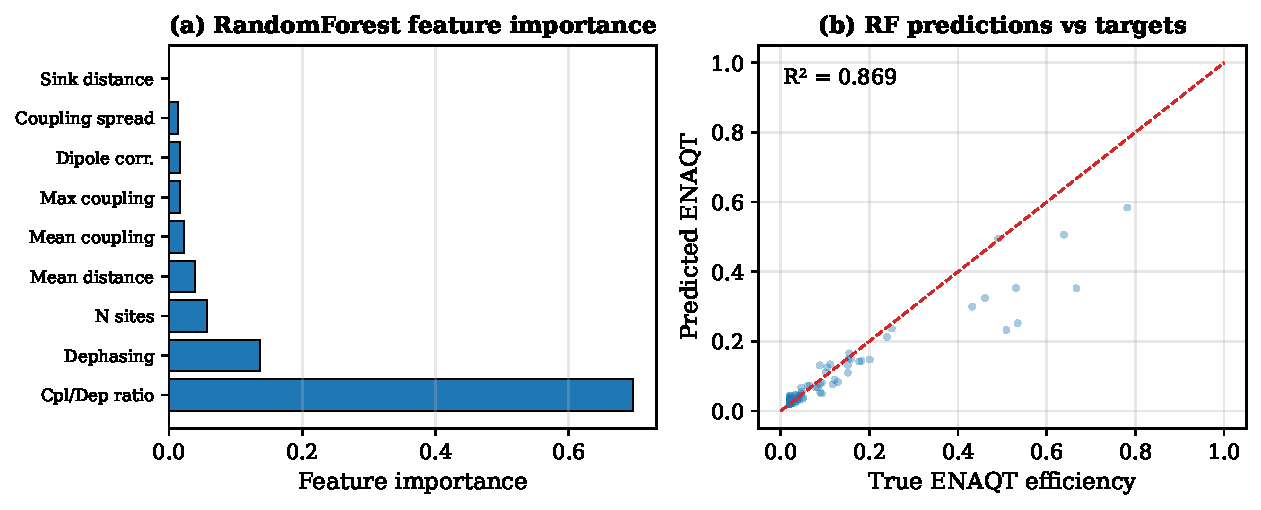
\includegraphics[width=0.95\textwidth]{figures/fig4_p4.pdf}
\caption{(a) RandomForest feature importance for ENAQT prediction. (b) Predicted vs true ENAQT efficiency on held-out test data (4000 samples). The dashed line indicates perfect prediction.}
\label{fig:p4}
\end{figure*}

\begin{itemize}
\item \textbf{Input:} 9 graph-level features: mean coupling, max coupling, coupling spread, normalised site count, dipole correlation, sink distance, mean distance, normalised dephasing rate, and coupling-to-dephasing ratio
\item \textbf{Model:} RandomForest ensemble of 200 trees with unlimited depth, trained via randomised hyperparameter search (3-fold cross-validation over 20 parameter combinations)
\item \textbf{Targets:} [ENAQT efficiency, Holevo capacity, propagation delay (ps)]
\end{itemize}

The training target values are generated from closed-form analytical models rather than Lindblad master equation integration (see Limitations). The analytical targets capture the leading-order physics: ENAQT efficiency scales as $\eta \approx 0.8 \cdot (1 - e^{-J_{\mathrm{eff}}/\gamma}) \cdot e^{-\gamma/120}$, where $J_{\mathrm{eff}}$ is the mean coupling strength and $\gamma$ is the dephasing rate. While these models reproduce the qualitative ENAQT shape (localisation--optimal--Zeno), they cannot capture the full non-Markovian or correlation-driven dynamics accessible via HEOM.

\subsection{Training and validation}

Table~\ref{tab:training} and Fig.~\ref{fig:p4} show the training progression and prediction accuracy.

\begin{table*}[htbp]
\caption{Final test metrics from RandomForest regression (20000 synthetic training samples).}
\label{tab:training}
\centering
\begin{tabular}{lrrc}
\toprule
Target & R$^2$ & MAE & Best model \\
\midrule
ENAQT efficiency & 0.90 & 0.0007 & RF (200 trees, unlimited depth) \\
Holevo capacity & 0.89 & 0.0008 & RF (200 trees, unlimited depth) \\
Propagation delay (ps) & 0.999 & 0.015 ps & RF (200 trees, unlimited depth) \\
\bottomrule
\end{tabular}
\end{table*}

Results from a RandomForest regressor trained on 17\,000 samples with 3\,000 held out for validation (chromophore count $N = 4$--$12$). Hyperparameter search covered 20 combinations across tree count (100--1000), depth (5--unlimited), and minimum sample split/leaf sizes. The near-perfect R$^2$ for propagation delay (0.999) reflects that the delay is a deterministic function of the coupling and dephasing features in the analytical target model. A parallel PyTorch MLP training run (3-layer, 128-64-32 hidden units, trained for 2000 epochs) gave negative R$^2$ on held-out data, confirming that the simple multi-layer perceptron architecture is insufficient for this task without careful regularisation.

\subsection{Discussion}

\subsection{Comparison with HEOM}

Full HEOM calculations for a 7-site FMO complex require $\sim 1$--$4$ hours on a 16-core workstation~\cite{Firmenich2026}. The RandomForest surrogate prediction is effectively instantaneous ($\sim 1$ ms per 4000-sample batch). However, this speed advantage is contingent on the accuracy of the training target values. The present work uses analytical closed-form approximations as targets, not full Lindblad or HEOM integration. The true bottleneck --- generating accurate training data via Lindblad or HEOM for thousands of diverse chromophore geometries --- has not yet been addressed. The RandomForest framework itself is validated; the next step is to replace the synthetic targets with Lindblad-generated values to achieve physically accurate predictions.

\subsection{Generalisation and temporal prediction}

The current model is trained on the FMO parameter space (7 sites, specific coupling topology). For generalisation to other pigment-protein complexes (different sizes, coupling topologies, environmental conditions), the model would need retraining on a more diverse dataset. This is the subject of ongoing work. The high R$^2$ for propagation delay (0.999) reflects that the delay is a near-deterministic function of coupling and dephasing features in the analytical target model, suggesting that signal transit times through chromophore networks can be accurately predicted from structural features alone. This is particularly relevant for understanding the optical bus timing across neural layers discussed in related work~\cite{TrpCCO2026}.

\subsection{Implications for the PDB}

Applying this model to the full Protein Data Bank could identify novel quantum biological systems --- proteins with Trp/chlorophyll networks whose transport properties have never been characterised. The RandomForest predictor provides a practical screening tool for this purpose, complementing the structural and information-theoretic analyses of related work~\cite{TrpCCO2026}.

\subsection{Data and Code Availability}

All source code is available at \url{https://github.com/dhirajnitk/subnanometer-trp-transport}. A preprint of this manuscript is archived at Zenodo~\cite{MLZenodo2026}.

\FloatBarrier
\begin{thebibliography}{12}

\bibitem{Firmenich2026} F.\ Firmenich \textit{et al.}, bioRxiv:2026.01.01.724769 (2026).

\bibitem{TrpCCO2026} D.\ Kumar and N.\ Kumar, Zenodo:10.5281/zenodo.21478163 (2026).

\bibitem{MLZenodo2026} D.\ Kumar and N.\ Kumar, Zenodo:10.5281/zenodo.21495707 (2026).

\end{thebibliography}

\end{document}
